%\chapter{Lluvias atmosf\'ericas extendidas}
%\chapter{Lluvias atmosf\'ericas hadrónicas y de neutrinos}
\chapter{Búsqueda de neutrinos cósmicos mediante lluvias atmosféricas}
\label{ch:easAuger}

En este capítulo se presentan las estrategias de búsqueda de neutrinos cósmicos ultra energéticos utilizadas por el Observatorio Pierre Auger. En primer lugar se discute la producción de lluvias de partículas producidas por la interacción de rayos cósmicos en la atmósfera. A continuación se analizan las diferencias entre lluvias iniciadas por hadrones y por neutrinos. Por último se describen los tres canales utilizados por el experimento para la búsqueda de lluvias atmosf\'ericas extendidas generadas por neutrinos. 

%se discute la medición de rayos cósmicos a través de las lluvias de partículas que producen al interactuar en la atmósfera, se analizan las diferencias entre lluvias iniciadas por hadrones y por neutrinos, y se presentan las estrategias de búsqueda de neutrinos utilizadas por el Observatorio Pierre Auger.

\section{Lluvias atmosf\'ericas extendidas}

A fines de la década del treinta Pierre Auger observó que la coincidencia de disparo entre detectores de rayos c\'osmicos separados varios kilómetros era mayor a la esperada si se supon\'ia que los eventos eran independientes.
Explicó este hecho postulando la existencia de partículas muy energéticas que al interactuar en la alta atmósfera pudieran generar nuevas partículas de alta energía capaces, a su vez, de repetir el proceso. De esta manera se inicia un proceso de multiplicación en cadena que lleva hoy el nombre de lluvia atmosférica extendida (EAS, por su sigla en inglés). 

Al cabo de 70 años de investigación, la estructura y evolución de las cascadas atmosféricas se considera bien comprendida.
Tras la primera interacción, su desarrollo puede describirse como un núcleo de partículas de alta energía (usualmente hadrones), que avanza a lo largo del eje de la lluvia produciendo electrones, muones y fotones menos energéticos.
Estas part\'iculas secundarias poseen mayor momento transverso relativo, por lo que difunden en la dirección radial (ver figura~\ref{fig:lluvia1}). Así, las cascadas se constituyen por tres componentes: hadrónica, muónica y electromagnética (ver figura~\ref{fig:showerSchema}), aunque la estructura detallada depende de gran cantidad de factores como por ejemplo partícula primaria, su energ\'ia o profundidad de la interacción inicial.

%
\begin{figure}[ht]
\begin{center}
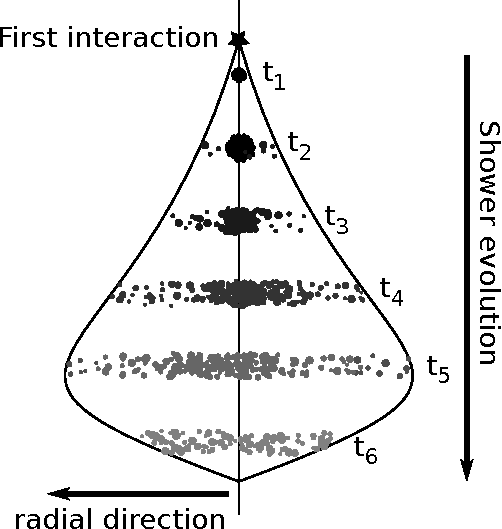
\includegraphics[width=0.75\textwidth]{fig/EASAuger/lluvia1_english.pdf}
\caption{Esquema de la evolución de una cascada atmosférica. Tras la primera interacción se forma un núcleo de partículas de alta energía (usualmente hadrones), que avanza a lo largo del eje de la lluvia produciendo nuevas partículas menos energéticas pero con mayor momento transverso relativo, que difunden en dirección radial.}
\label{fig:lluvia1}
\end{center}
\end{figure}
%
%
\begin{figure}[ht]
\begin{center}
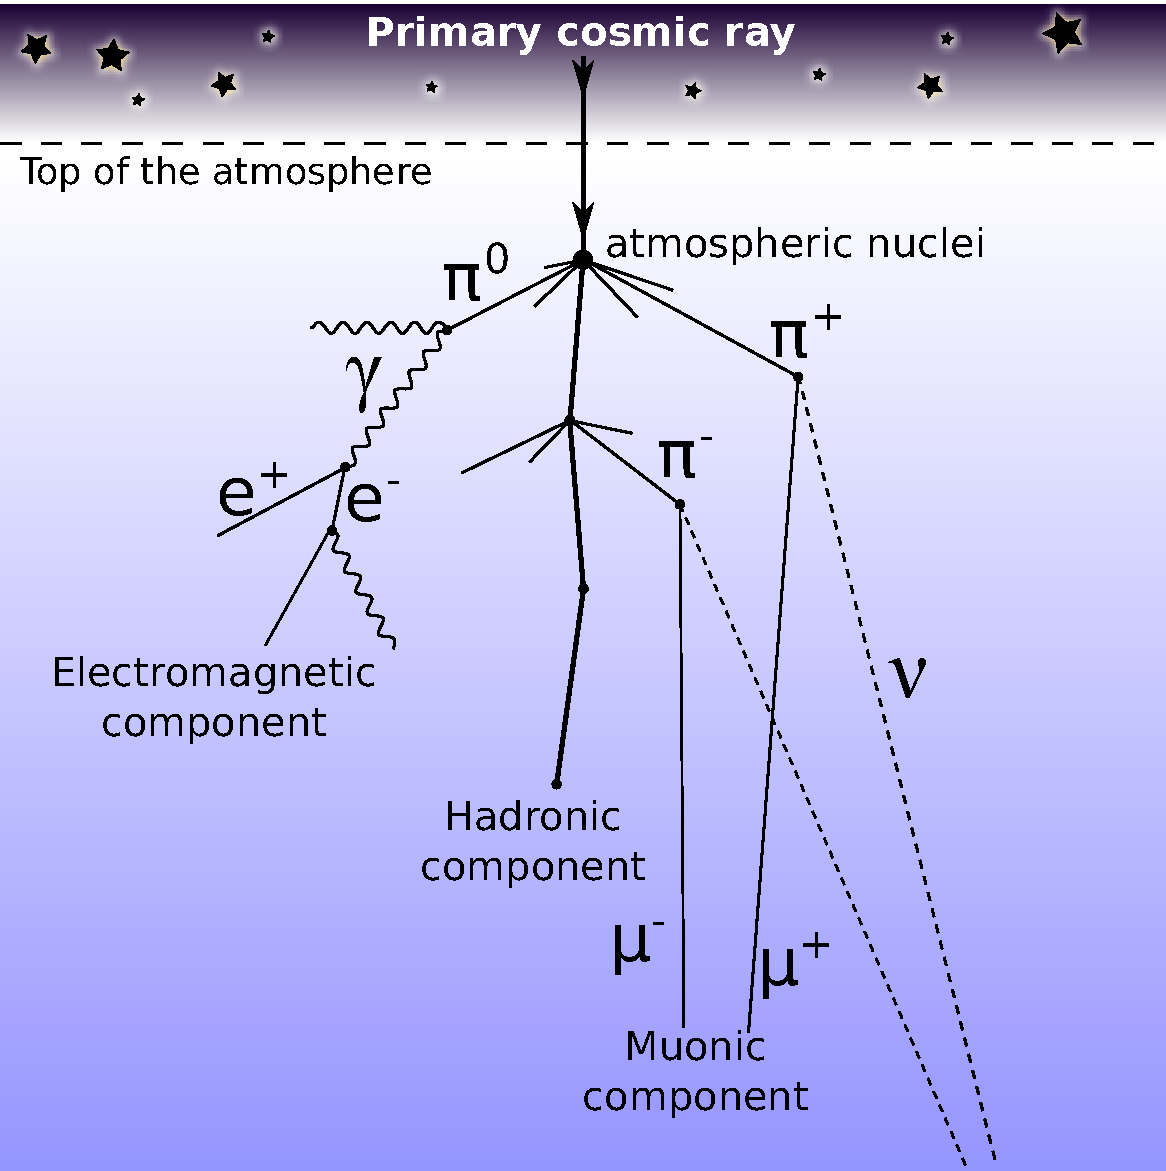
\includegraphics[width=0.75\textwidth]{fig/EASAuger/showerSchema_english.pdf}
\caption{Diagrama esquemático de la estructura de una cascada atmosférica.}
\label{fig:showerSchema}
\end{center}
\end{figure}
%

En la actualidad se considera que la gran mayoría de las cascadas con energía superior a $10^{16}$~eV son iniciadas por UHECR hadrónicos \cite{CONSEGUIR}. 
En estas lluvias, el número de hadrones aumenta rápidamente durante las primeras etapas de la cascada, predominando la generaci\'on equiprobable de $\pi^{0}$, $\pi^{+}$ y $\pi^{-}$,por simetría de isospin.
Dado de que el decaimiento del $\pi^{0}$ es 100\% electromagnético ($98.823\pm0.034\%$ a $\gamma\gamma$ y $1.174\pm0.035\%$ a $e^+e^-\gamma$~\cite{Agashe:2014kda}), en cada generación un tercio de la energía de la componente hadr\'onica es transferida a la componente electromagnética.

Por otro lado, la energ\'ia entregada a la componente muónica de la lluvia crece más lentamente. 
Si bien el decaimiento de piones cargados produce exclusivamente muones ($99.98770\pm0.00004\%$ a $\mu^{\pm}\nu_\mu$~\cite{Agashe:2014kda}), debido a la dilatación temporal los $\pi^{\pm}$ más energéticos tienen menor probabilidad de decaer que de interactuar con un n\'ucleo atmosf\'erico, desarrollando así inicialmente la componente hadrónica.

En las etapas finales de la cascada alrededor del 90\% de la energía de la partícula primaria es disipada por la componente electromagnética mediante ionización. La restante es transportada por los muones y neutrinos provenientes del decaimiento de los piones menos energéticos.

\section{Lluvias iniciadas por hadrones}
En esta sección se presenta una descripción simplificada de las lluvias atmosféricas, desarrollado originalmente por Heitler \cite{hei54} a mediados de los años 50. Si bien es demasiado simple para obtener resultados cuantitativos precisos, ayuda a comprender cualitativamente la dinámica de las lluvias.

\subsection{Componente electromagnética}
En el cálculo de la evolución de la porción electromagnética de la lluvia se asume que cada electrón radía por bremsstrahlung un único fotón después de viajar una distancia $d=\lambda \ln 2$, donde $\lambda\simeq38$~g~cm$^{-2}$ es la longitud de radiación propia del medio\footnote{Aqu\'i $d$ es la distancia promedio en que un electrón irradia la mitad de su energía.}. Simultáneamente se propone que cada fotón producirá un par $e^{-}$ $e^{+}$ después de recorrer esta misma distancia.
Este proceso se esquematiza en la figura \ref{fig:heilter}.
%
\begin{figure}[ht]
\begin{center}
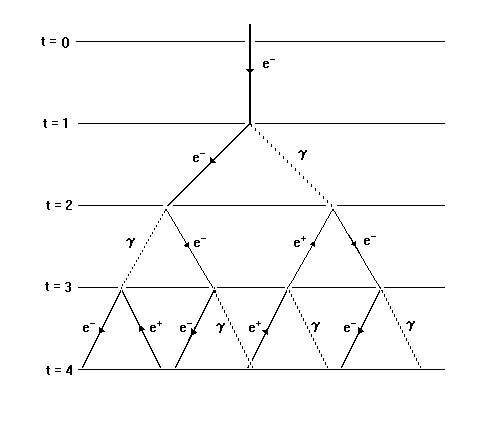
\includegraphics[width=0.75\textwidth]{fig/EASAuger/heilterSchema}
\caption{Esquema del modelo de Heilter. Luego de cada longitud de radiación ($t=nd/\lambda$) los $e^\pm$ emiten un fotón, mientras que los fotones producen un par $e^+e^-$.}
\label{fig:heilter}
\end{center}
\end{figure}
%
En ambos casos se toma que la energía se reparte equitativamente entre las partículas hijas. Después de $n$ pasos la lluvia contará con $2^{n}$ partículas entre electrones, positrones y fotones. El modelo considera que la generación de nuevas partículas se detiene cuando la energía perdida por colisiones\footnote{Es decir, ionizaci\'on y excitaci\'on de las mol\'eculas del aire, esencialmente $N_2$ y $O_2$.} es mayor que la necesaria para los procesos de bremsstrahlung y producción de pares. En el aire esta energía de corte es de aproximadamente \cant{85}{MeV}. En este punto la cantidad de partículas es máxima y valen las siguientes ecuaciones:
%
\begin{equation}
\label{hi1}
E_p = E_{corte} N_{max} = E_{corte} 2^{n_{max}}
\end{equation}
%
\begin{equation}
\label{hi2}
X_{max}=n_{max} d
\end{equation}
%
con $X_{max}$ la coordenada donde la lluvia alcanza la máxima cantidad de partículas $N_{max}$ luego de $n_{max}$ pasos y $E_p$ la energía del primario.
Despejando $n_{max}$ de (\ref{hi1}) y reemplazando en (\ref{hi2}) se obtiene para $X_{max}$:
%
\begin{equation}
\label{hi3}
X_{max} = n_{max} \lambda \ln2=\lambda \ln\left(\frac{E_{0}}{E_{corte}}\right)
\end{equation}
%
Pese a la simplicidad del modelo, las relaciones \ref{hi1} y \ref{hi3}, que pueden a su vez resumirse en \ref{hi4}, describen correctamente los resultados alcanzados mediante simulaciones más sofisticadas a partir de primeros principios.
%
\begin{equation}
\label{hi4}
X_{max} \sim \ln E_{p}
\hspace*{15mm}
N_{max} \sim E_p
\end{equation}
%

\subsection{Componente hadrónica y muónica}

Para modelar la componente hadrónica de la lluvia es posible utilizar un esquema similar al empleado para estudiar la electromagnética.
Se considera que la totalidad de los hadrones son piones ($\pi^{\pm}$ y $\pi^{0}$). Los $\pi^{\pm}$ al interactuar con n\'ucleos de la atm\'osfera generan $N \pi^{\pm}$ y $\frac{1}{2}N \pi^{0}$ después de atravesar una feta de atmósfera de ancho $d=\lambda \ln2$ siendo $\lambda$ la longitud de interacción para partículas que interactúan fuertemente.
Los $\pi^{0}$ decaen inmediatamente en dos fotones que pasan a formar parte de la componente electromagnética y los $\pi^{\pm}$ continúan la cascada hadrónica hasta que su energía no les permite generar nuevos piones.
En este punto los $\pi^{\pm}$ s\'olo pueden decaer a muones.
Estos muones, provenientes de $\pi^{\pm}$ de baja energía, forman la totalidad de la componente muónica de la lluvia.
El alto poder de penetración de los muones les permite atravesar la atmósfera sin interactuar en el camino, por lo que generalmente alcanzan la superficie de la Tierra antes que la componente electromagnética.

\subsection{Lluvias inclinadas}
\label{sbsc:inclinadas}
%
El término ``lluvias inclinadas'' se refiere a lluvias cuyo ángulo cenital $\theta$ es mayor a $60^{\circ}$.
Con el fin de motivar esta definición es interesante estudiar la cantidad de materia que la lluvia tiene que atravesar hasta alcanzar la Tierra como función de $\theta$.
En la figura \ref{fig:slant_depth} se muestra como entre $0^{\circ}$ y $60^{\circ}$ el cambio en la profundidad es un factor $\sim 2$ respecto de su contraparte vertical, \cant{\sim1000}{g/cm^{2}}.
A partir de este punto la profundidad crece rápidamente, alcanzando un factor $\sim 36$ a $\theta=90^{\circ}$.
%
\begin{figure}[h!]
\begin{center}
$
\begin{array}{cc}
 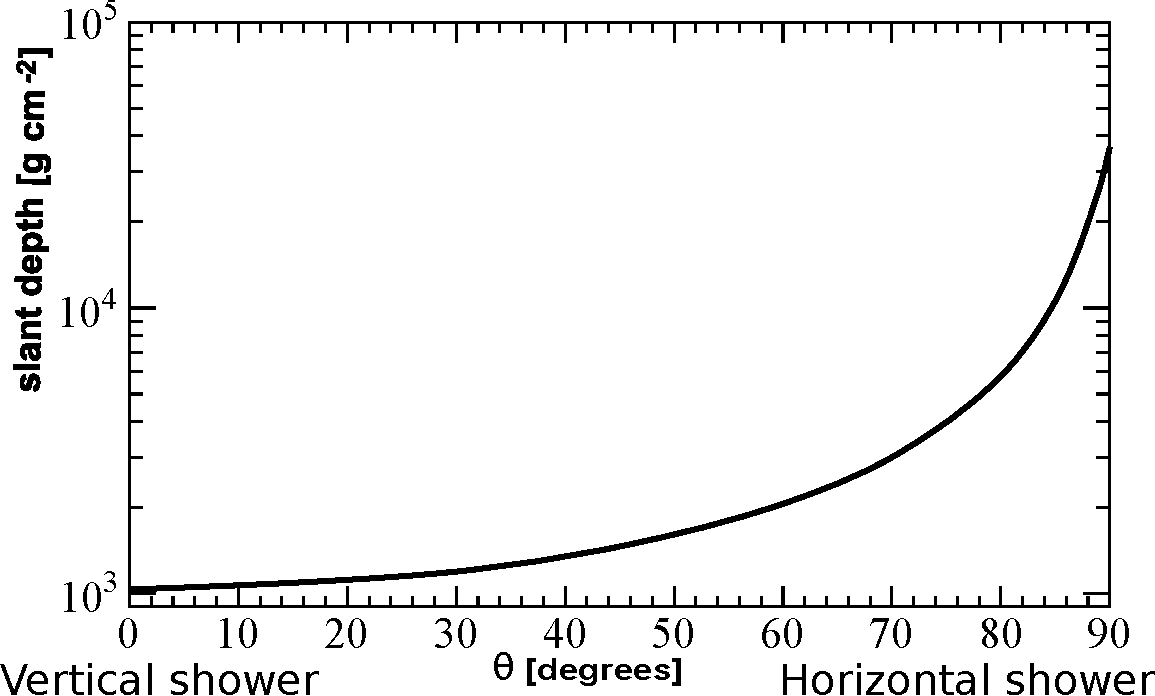
\includegraphics[width=0.47\textwidth]{fig/EASAuger/slant_depth_english.pdf} & 
 \raisebox{0.8\height}{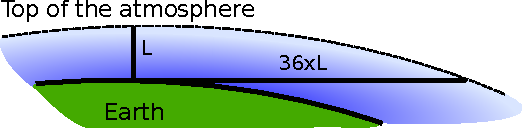
\includegraphics[width=0.47\textwidth]{fig/EASAuger/slantCartoon_english.pdf}}
\end{array}
$
\caption{\textit{Izquierda:} Profundidad atmosférica como función del ángulo cenital $\theta$.
La cantidad de materia crece rápidamente para $\theta\gtrsim60^{\circ}$.
\textit{Derecha:} Una lluvia completamente horizontal atraviesa 36 veces más materia que una vertical.
}
\label{fig:slant_depth}
\end{center}
\end{figure}
%

La mayor parte los rayos cósmicos con energías superiores a \cant{10^{16}}{eV} son protones o n\'ucleos.
Dado que su longitud de interacción en la atmósfera es \cant{\sim50}{g/cm^{2}}, es correcto considerar que estas interact\'uan en el tope de la atmósfera.
En consecuencia, para lluvias con $\theta>70^\circ$, tanto la componente hadrónica como la electromagnética son completamente absorbidas por la atmósfera\footnote{De la figura \ref{fig:effDG_tr_id} del cap\'itulo \ref{ch:resAuger} de esta Tesis puede deducirse que luego de \cant{2000}{g/cm^2} la componente electromagn\'etica es completamente absorbida por la atm\'osfera.}, por lo que sólo la componente muónica alcanza la superficie de la Tierra, lo que se esquematiza en la figura \ref{fig:horizontalHad}.
Como resultado, a nivel del suelo las lluvias horizontales son fundamentalmente diferentes de las verticales.
%
\begin{figure}[h!]
\begin{center}
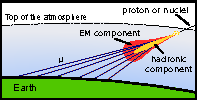
\includegraphics[width=0.7\textwidth]{fig/EASAuger/horizontal2_english.pdf}
\caption{Las lluvias inclinadas producidas por protones o n\'ucleos se inician cerca del tope de la atmósfera.
Las componentes hadrónica y electromagnética se absorben rápidamente, por lo que sólo los muones alcanzan el suelo.
}
\label{fig:horizontalHad}
\end{center}
\end{figure}

\section{Lluvias atmosf\'ericas iniciadas por neutrinos}
\label{sc:easNu}

Existen dos mecanismos predominantes mediante los cuales los neutrinos ultra energ\'eticos pueden iniciar lluvias atmosféricas extendidas capaces de producir una se\~nal medible por un detector de superficie.
Cada uno da lugar a un tipo diferente de evento, que ser\'an denominados a partir de aqu\'i como \emph{lluvias descendentes} o \emph{down going} (DG) y \emph{lluvias rasantes} o \emph{earth-skimming} (ES).
% Estos dan lugar a dos tipos de lluvias atmosf\'ericas, a saber:
% \begin{itemize}
%  \item Lluvias descendentes (DG, down going)
%  %Un neutrino deposita algo de su energía en la atmósfera generando una lluvia descendente cuyas partículas alcanzan el suelo.
%  \item Lluvias rasantes iniciadas por neutrinos \tauon{} (ES, earth-skimming)
%  %Un neutrino ascendente interactúa con la corteza de la tierra y alguno de sus productos de decaimiento genera una cascada en la atmósfera muy cerca del suelo.
% \end{itemize}

\subsection{Lluvias descendentes}
\label{sbsc:easDG}

% De acuerdo con el modelo estandar (SM por sus siglas en inglés), los neutrinos interactúan mediante la gravedad y la fuerza débil, pero sólo esta última puede ser utilizada para detectar neutrinos individuales.
Un neutrino que ingresa a la atm\'osfera interactuar\'a mayormante debido a la dispersión inelástica profunda (DIS por sus siglas en inglés, \emph{Deep Inelastic Scattering}) con los n\'ucleos de la misma.
Los posibles canales para esta interacci\'on discriminados por sabor de neutrino se esquematizan en la figura \ref{fig:SM_nu_int}.
En todos los casos, cerca del \cant{20}{\%} de la energía del primario se transfiere al jet hadrónico que se genera al fragmentarse el n\'ucleo atmosf\'erico.
Como resultado, se genera una cascada de características similares a las iniciadas por protones o núcleos.
Por otra parte, el \cant{80}{\%} de la energ\'ia restante se transfiere a un leptón ultra energético que según el caso puede contribuir o no a la EAS generada.
%
\begin{figure}[ht]
\begin{center}
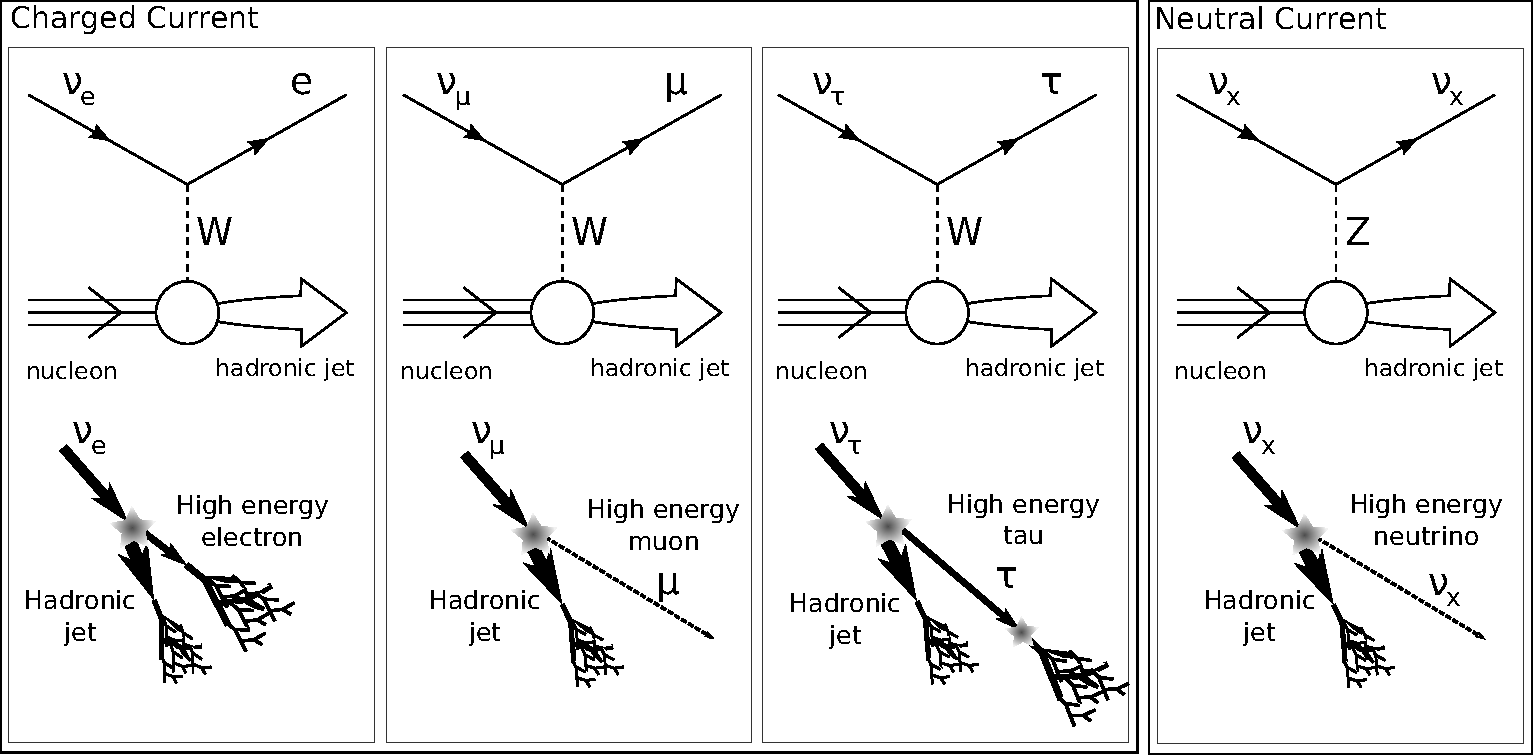
\includegraphics[width=1.0\textwidth]{fig/EASAuger/nu_channels_english.pdf}
\caption{Canales de interacción para neutrinos de acuerdo con el Modelo Estandar.
En todos los casos se muestra el diagrama de Feynman al orden más bajo.
Para todos los canales, el jet resultante de la fragmentación del núcleo inicia una lluvia hadrónica que posee alrededor del \cant{20}{\%} de la energía del neutrino incidente.
El electrón producido en la interacción via corriente cargada (CC) genera una cascada electromagnética que se suma al jet hadrónico.
Cuando el neutrino primario es un $\nu_{\tau}$ que interact\'ua via CC el $\tau$ generado puede viajar una distancia considerable antes de decaer y generar una cascada, a veces muy cercana al suelo.
Estas se denominan \emph{cascadas double bang}.
Finalmente, en el caso de tener un $\nu_{\mu}$ primario, el $\mu$ resultante en la mayor parte de los casos no genera lluvia alguna.
}
\label{fig:SM_nu_int}
\end{center}
\end{figure}

Cuando la interacci\'on se produce via corriente neutra (NC), luego de perder energía el neutrino escapa sin generar cascada alguna, transmiti\'endose a la lluvia sólo el \cant{20}{\%} de la energía del primario.
En cambio, si el evento es iniciado por un $\nu_e$ via corriente cargada (CC), el electrón resultante tambi\'en iniciar\'a una cascada electromagnética que se superpone con la hadrónica, generada por los fragmentos del núcleo.
En este caso, toda la energía del neutrino primario es transferida a la lluvia.

Aunque el mecanismo de interacci\'on primario difiere, los eventos iniciados por $\nu_{\mu}$ via CC son muy similares a las generados via NC, ya que las probabilidades de que el $\mu$ resultante de la interacción decaiga o interactúe antes de llegar al suelo son pequeñas\footnote{La probabilidad de que un $\mu$ de \cant{10^{18}}{eV} decaiga antes de llegar al suelo es de $\sim10^{-6}$ mientras que la probabilidad de que sufra DIS o bremsstrahlung es del orden de $10^{-3}$ \cite{cite:tesisJavier}}.

Por \'ultimo, en el caso de un $\nu_{\tau}$ que interactúa via CC al proceso se le agrega una particularidad.
Al igual que el $\mu$, el $\tau$ resultante es una partícula muy penetrante pero en este caso su vida media es siete \'ordenes de magnitud menor.
As\'i, luego de viajar una distancia apreciable\footnote{\cant{5}{km} para un $\tau$ de \cant{10^{17}}{eV}.} decaerá generando en el \cant{\sim80}{\%} de los casos una cascada detectable, que a su vez será el \cant{\sim25}{\%} de caracter electromagnético y el \cant{\sim75}{\%} restante hadrónico (ver cap\'itulo \ref{ch:simulacionAuger}).
Este tipo de cascadas, muy características, se conocen como ``Double--Bang'' (DB).
%
\begin{figure}[h!]
\begin{center}
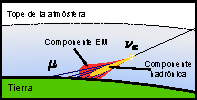
\includegraphics[width=0.7\textwidth]{fig/EASAuger/horizontal_deep_english.pdf}
\caption{Los neutrinos pueden iniciar lluvias inclinadas profundas en la atmósfera.
En este tipo de lluvias tanto la componente electromagnética como la muónica pueden llegar al suelo.
Comparar con la figura \ref{fig:horizontalHad}.
}
\label{fig:horizontalNu}
\end{center}
\end{figure}

Por otra parte, para cada \'angulo cenital la ubicaci\'on de interacci\'on primaria se distribuye exponencialmente.
El camino libre medio de esta distribuci\'on es por ejemplo, para neutrinos de \cant{10^{18}}{eV}, \cant{\sim10^8}{g/cm^{2}}\cite{cite:Gandhi}. 
Dado que este valor es mucho mayor que el espesor m\'asico de la atmósfera, incluso para $\theta\sim90^\circ$, es posible aproximar el decaimiento exponencial como una constante, o visto de otra manera, es aceptable considerar que los neutrinos pueden interactuar básicamente en cualquier punto de la atmósfera con la misma probabilidad.
Por este motivo, los neutrinos tienen la capacidad de iniciar lluvias lo suficientemente profundas como para que tanto la componente electromagnética como la muónica alcancen el suelo (ver figura \ref{fig:horizontalNu}).
Esta caracter\'istica es la que permite distinguir los eventos iniciados por neutrinos de las lluvias hadr\'onicas regulares utilizando detectores de superficie.
La estrategia utilizada se basa en la identificaci\'on de lluvias inclinadas en las que la componente electromagnética no haya sido absorbida por la atmósfera, lo que da lugar al canal de detección que denomina Down-going (DG).

%
\subsection{Lluvias rasantes}
\label{sc:EStauInducedShowers}
%
Al igual que en la atm\'osfera, un neutrino que atraviesa la Tierra puede interactuar mediante DIS con alguno de sus n\'ucleos.
En este proceso, tanto el jet hadrónico producido como el electrón producido, en el caso de un $\nu_e$ incidente, son rápidamente absorbidos por la materia.
Sin embargo, los leptones $\mu$ y $\tau$ producidos al incidir un $\nu_{\mu}$ o un $\nu_{\tau}$ pueden escapar hacia la atm\'osfera gracias a su baja sección eficaz.
Los $\mu$ que emerjan de la Tierra poseerán una vida media tal que en la mayor\'ia de los casos, la lluvia atmosf\'erica iniciada en su decaimiento se producir\'a muy alto en la atmósfera.
Por este motivo, las partículas secundarias generadas rara vez alcanzarán el suelo.
Como contraparte los leptones $\tau$ poseen un tiempo de vida media que les permite decaer cerca de la superficie\footnote{La longitud de decaimiento es $\lambda_{d}=c\tau_{\tau}\gamma_{\tau}=49\,\text{km}\times\frac{E_{\tau}}{\text{EeV}}$} e iniciar una cascada detectable.
Si bien las part\'iculas de la misma se desplazar\'an en promedio hacia arriba, si el \'angulo cenital es lo suficientemente rasante ($\sim 90^\circ-95^\circ$) una cantidad suficiente alcanzar\'a el suelo pudiendo as\'i disparar un detector de superficie.
Este canal de detección, que se esquematiza en la figura \ref{fig:esNu}, es utilizado por los experimentos de rayos c\'osmicos en la b\'usqueda de neutrinos ultra energ\'eticos y se denomina Earth-Skimming (ES).

\begin{figure}[ht]
\begin{center}
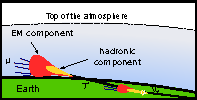
\includegraphics[width=0.7\textwidth]{fig/EASAuger/horizontal_es_english.pdf}
\caption{Un $\nu_{\tau}$ puede interactuar en la Tierra via CC dando como resultado un $\tau$ que puede emerger a la atmósfera e iniciar una EAS muy cerca de la superficie.
Aunque \'esta es ascendente, si el $\tau$ emergente posee un ángulo cenital entre $90^\circ$ y $95^\circ$ las partículas que llegan al suelo suelen ser suficientes para detectar la lluvia.}
\label{fig:esNu}
\end{center}
\end{figure}

% Dado que la densidad de la corteza terrestre es $\sim1000$ veces mayor a la del aire, funciona como un blanco muchísimo mas masivo que la atmósfera para los neutrinos.
% Como ejemplo, el camino libre medio para un neutrino de \cant{10^{18}}{eV} en la Tierra\footnote{la densidad de la Tierra es \cant{\rho\sim2.65}{\frac{g}{cm^3}}} es de \cant{\sim620}{km}.
% Por otro lado, bajo la aproximación de Tierra esférica, la distancia que debe recorrer un neutrino para atravezarla es $d\sim2R\cos{\theta}$, donde $R$ es el radio de la Tierra. 
% En consecuencia, como para $91^{\circ}$ se obtiene \cant{d\sim220}{km}, se concluye que \cant{\sim30}{\%} de los neutrinos interactuarán en esas condiciones.
% Luego, es necesario considerar la probabilidad de que el $\tau$ escape de la Tierra sin perder demasiada energía y a su vez decaiga lo suficientemente cerca del suelo, pero esto se analizará en detalle en la sección \ref{sc:pesos}.

\section{Canales de búsqueda de neutrinos}

El m\'aximo desafío para detectar neutrinos cósmicos de UHE utilizando detectores de superficie es identificar los eventos que éstos inician en medio del inmensamente más poblado fondo de lluvias hadrónicas. Esto puede lograrse para eventos inclinados separando las lluvias jóvenes, es decir, aquellas con presencia de componente electromagn\'etica.

La figura \ref{fig:augerNu} resume los distintos tipos de lluvias discutidos.
Debido a sus diferentes características, en Auger se desarrollaron tres búsquedas optimizadas para distintos rangos de ángulo cenital:
\begin{itemize}
   \item DGL (Down Going Low): optimizado para neutrinos descendientes con ángulos entre $60^\circ$ y $75^\circ$.
   \item DGH (Down Going High): como DGL pero para lluvias muy inclinadas, con ángulos entre $75^\circ$ y $90^\circ$. 
   \item ES (Earth Skimming): optimizado para detectar neutrinos que inciden rasantes, cuyo ángulo se encuentre entre $90^\circ$ y $95^\circ$.
\end{itemize}
	\begin{figure}[ht!]
		\centering
		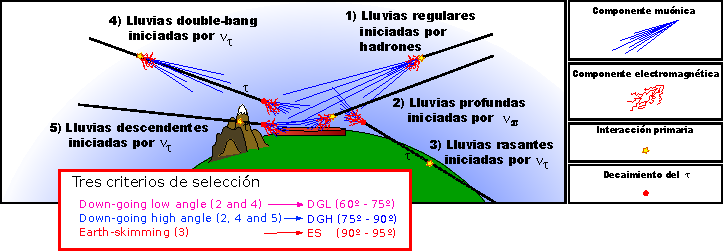
\includegraphics[width=\textwidth]{./fig/estrategiaAuger/auger_nu}
		% curveEarthSketch.png: 2404x1199 pixel, 150dpi, 40.70x20.30 cm, bb=0 0 1154 575
		\caption{\label{fig:augerNu}
		Esquema de los canales de detección de neutrinos con el SD del Observatorio Pierre Auger. Se detallan los tres análisis que fueron optimizados para identificar neutrinos provenientes de los diferentes rangos angulares.
		}
	\end{figure}
%
%Cada uno de estos an\'alisis ha dado lugar a una Tesis doctoral. DGL fue encarado por Jos\'e Luis Navarro en el grupo de la Universidad de Granada~\cite{cite:tesisNavarro}. Mientras que DGH y ES han sido tomados por el grupo de la UBA, dando lugar a las Tesis doctorales de Javier Tiffenberg~\cite{cite:tesisJavier} y Yann Guardincerri~\cite{cite:tesisYann}.

	El canal DGL fue analizado por el grupo de la Universidad de Granada, y es parte de la Tesis doctoral de Jos\'e Luis Navarro~\cite{cite:tesisNavarro}. El análisis DGH fue desarrollado en la UBA por Javier Tiffenberg y Yann Guardincerri, y está detallado en la Tesis del primero~\cite{cite:tesisJavier}. El canal ES fue al comienzo explorado por el grupo de la Universidad de Paris VI~\cite{cite:propagaTierra}, y luego desarrollado en la UBA en el marco del doctorado de Yann Guardincerri~\cite{cite:tesisYann} y la presente Tesis. 

En los tres casos, la estrategia utilizada para la búsqueda fue del tipo \emph{análisis ciego}. Este consiste primero en establecer un criterio de selección, mediante el cual se decide si un evento es candidato a neutrino o no. Para ello se utilizan simulaciones de lluvias de neutrinos (capítulo~\ref{ch:simulacionAuger}) y una pequeña fracción de los datos (capítulo~\ref{ch:selAuger}). Una vez definido el criterios de identificación, y determinada su contaminación y eficiencia (capítulo~\ref{ch:resAuger}), recién entonces se aplica la búsqueda sobre (la fracción dominante de) los datos.
Se denomina análisis ciego precisamente porque todo el estudio se realiza sin ``mirar'', hasta el último momento, los datos utilizados para la búsqueda.

Por último, y para potenciar la sensitividad de la búsqueda, como parte de esta Tesis se realizó un análisis conjunto de los tres canales, analizando en detalles sus eficiencias e incertezas experimentales, y combinándolos en un único resultado.


%%%%%%%%%%%%%%%%%%%%%%%%%%%%%%%%%%%%%%%%%%%%%%%%%%%%%%%%%%%%%%%%%%%%%%%%
\if{0}
El procedimiento se esquematiza en la figura \ref{fig:strAuger}. 
%
\begin{figure}[ht!]
	\centering
	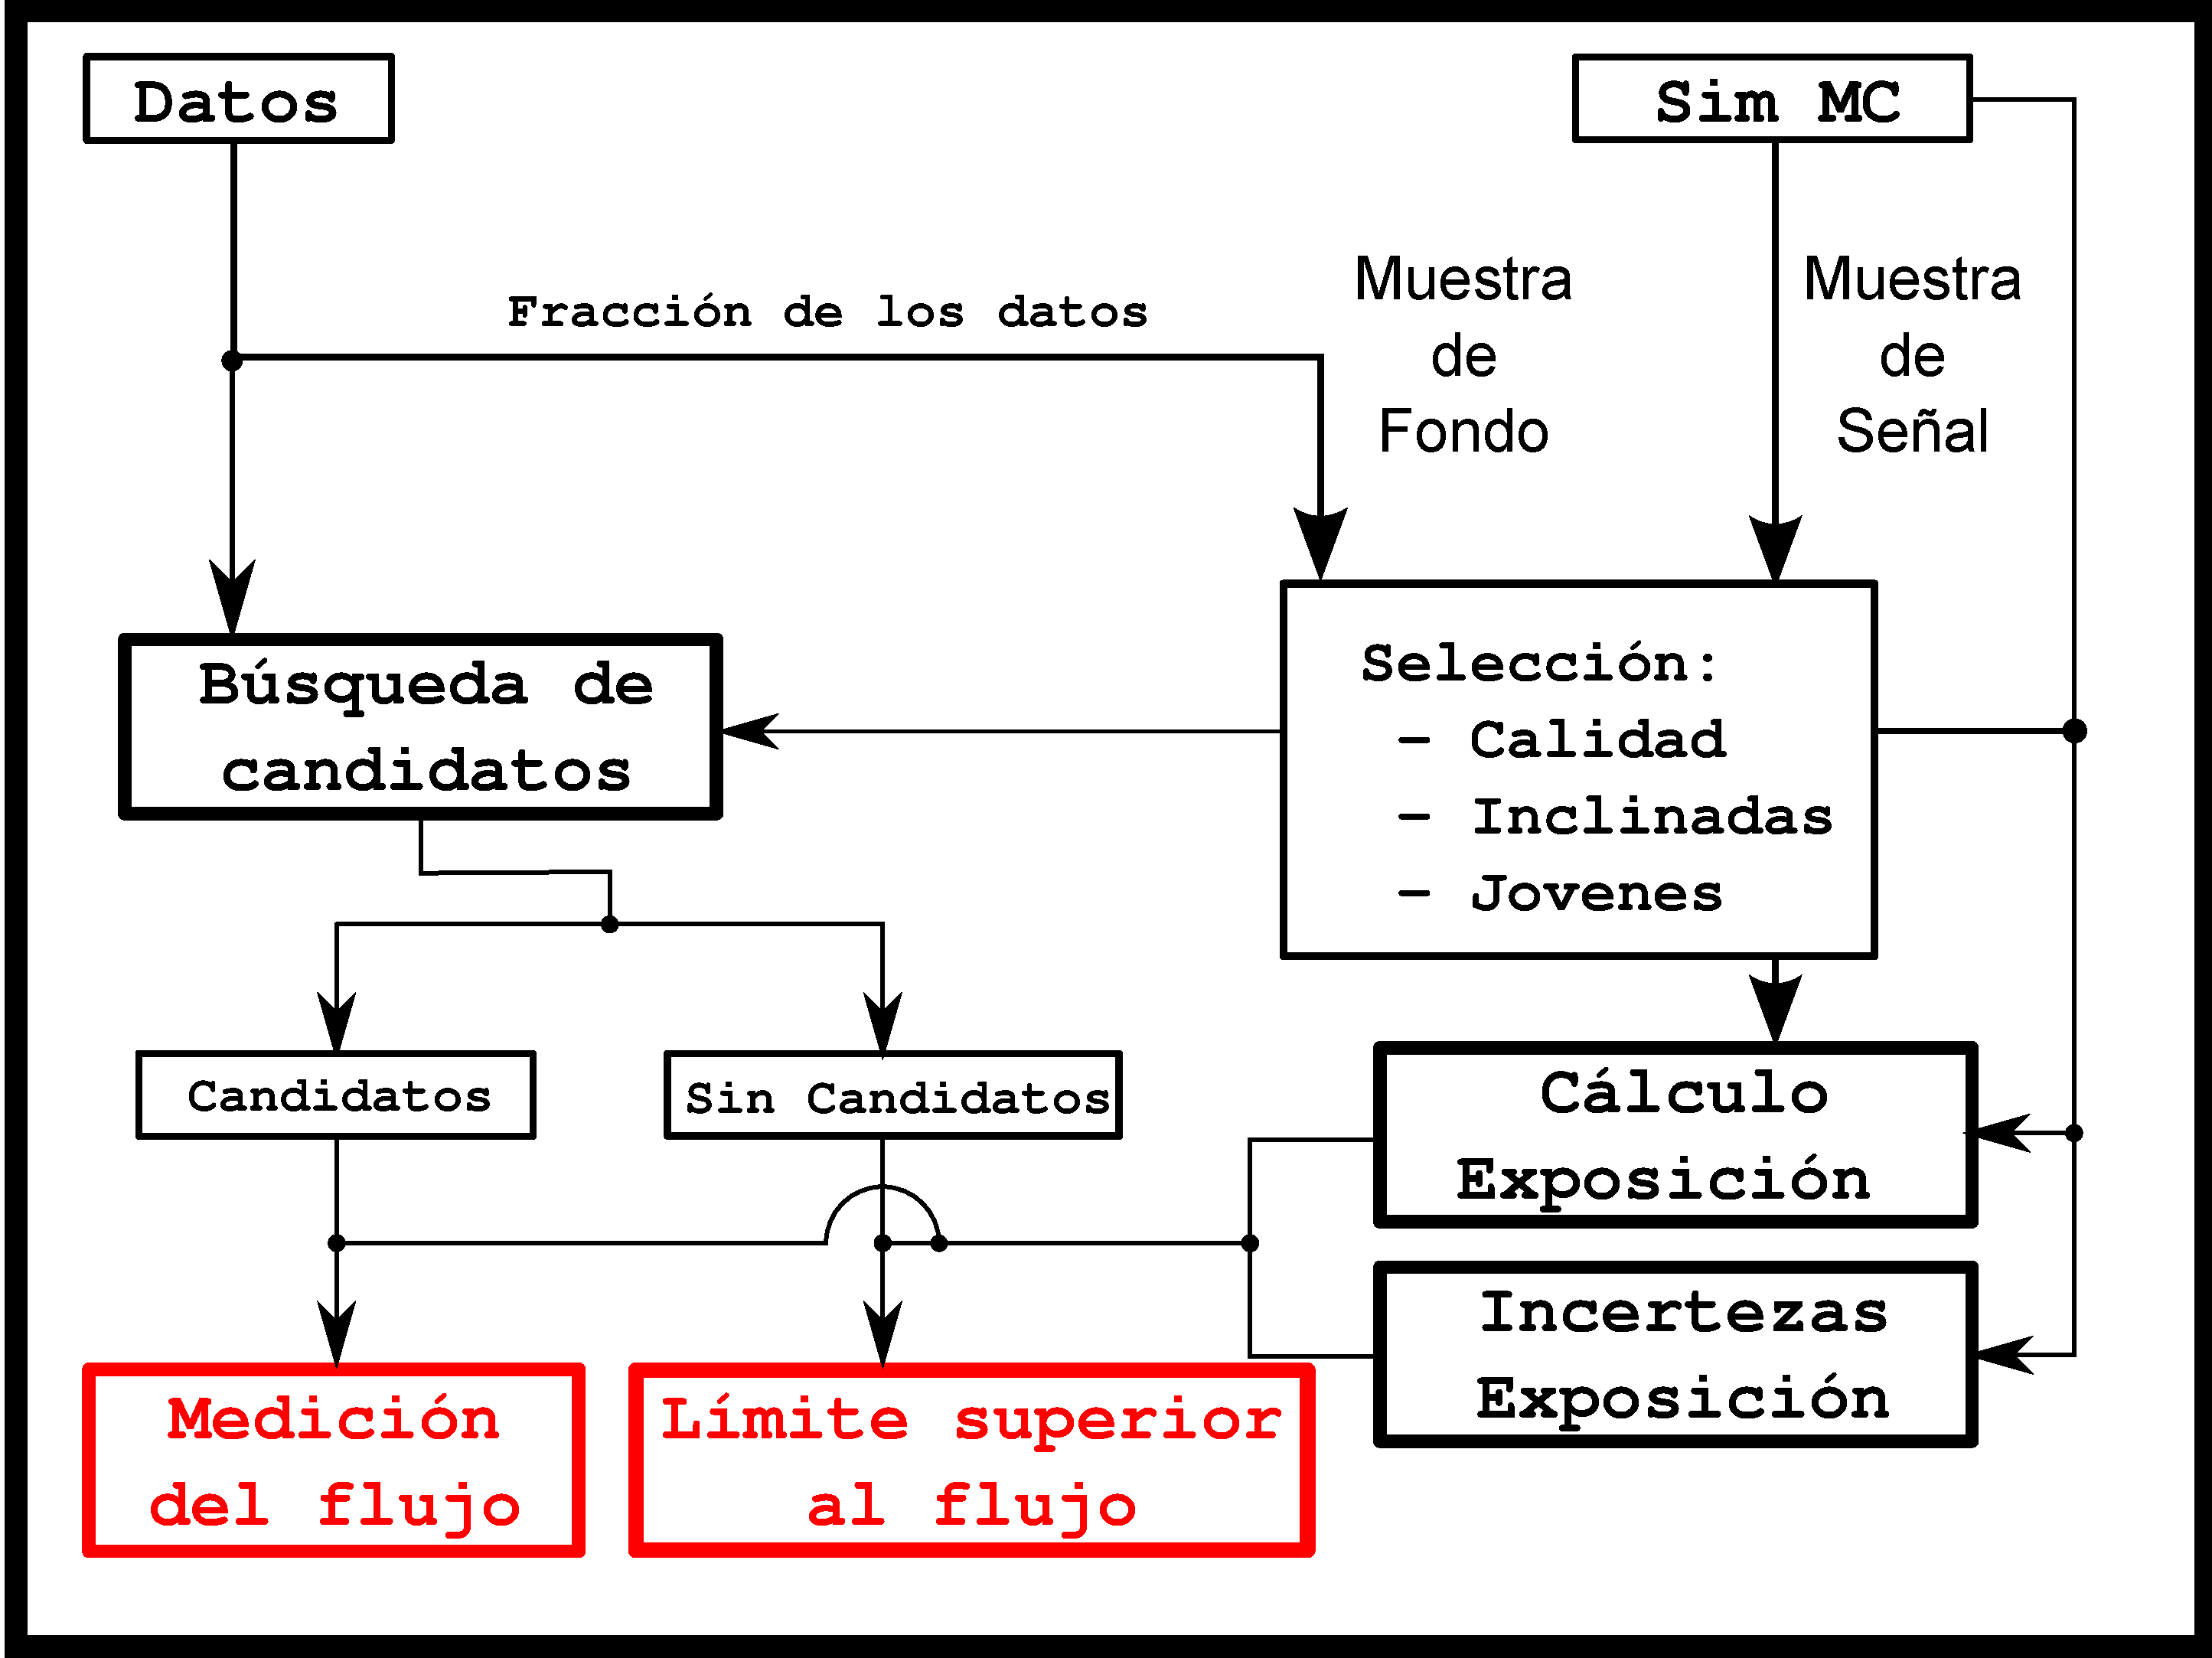
\includegraphics[width=\textwidth]{./fig/estrategiaAuger/analysisSchema}
	\caption{\label{fig:strAuger}
	Esquema de la estrategia utilizada en las búsquedas de neutrinos con el Observatorio Pierre Auger. Ver la explicación en el texto.
	}
\end{figure}
%
Aqu\'i la idea principal consiste en definir un criterio de selección, mediante el cual se decide si un evento es candidato a neutrino o no, sin utilizar datos o empleando una fracción peque\~na de los mismos que luego no podrá ser utilizada para realizar la búsqueda.
Luego es posible, por un lado, calcular con sus incertezas sistemáticas la exposición del detector a los distintos tipos de neutrinos, y por el otro, realizar la búsqueda de candidatos sobre los datos que no fueron utilizados en el entrenamiento del criterio.
Si hubiese candidatos en la muestra de b\'usqueda, sería posible informar la magnitud de el flujo con su error, o en caso contrario imponer un l\'imite superior a su valor.

Cabe destacar que para educar el criterio de selección es necesario contar con una muestra de señal (neutrinos) y otra de fondo (no neutrinos).
En los tres análisis se utilizaron simulaciones de Monte Carlo para generar la muestra de señal y una fracción de los datos como muestra de fondo.
% Este procedimiento, que emplea una parte de los datos para entrenar el m\'etodo, es lícito si los mismos son en su inmensa mayor\'ia no neutrinos y si el m\'etodo de entrenamiento no es sensible a outliers, condiciones que se satisfacen en los tres an\'alisis de Auger.
Luego, con las muestras de señal y fondo, se definieron criterios de calidad con el fin de eliminar eventos espureos y se optimizaron cortes en diferentes variables del detector que permiten elegir las lluvias jóvenes entre las inclinadas. 

En los próximos capítulos se abordarán las distintas etapas del análisis para las tres búsquedas.
Tambi\'en se presentar\'a su combinaci\'on y el c\'alculo de una \'unica exposici\'on a neutrinos ultra energ\'eticos con el Observatorio Pierre Auger.

\fi
%%%%%%%%%%%%%%%%%%%%%%%%%%%%%%%%%%%%%%%%%%%%%%%%%%%%%%%%%%%%%%%%%%%%%%%


